% slides-new: the showstopper deck with the motivation of questions-answers.tex,
% section 8: the extremal mass is read at infinity; Psi is the potential
% conjugate to alpha, and its T->0 limit tests the entropy-extremality relation.
% Build: ./build-new.sh
% Showstopper deck: slides 1-5 dark, one headline each. Five-minute talk: five timed slides (title, question, result, validation, lessons)
% followed by a closing slide and five backup slides (appendix), not timed. Build: ./build.sh
% Every number on the slides is copied from manuscript/numbers.tex,
% short-summary/comparison-numbers.tex or prompts/uso-de-tiempo-y-tokens.md;
% the two derived ones (+31%, 2.3x) are asserted in make_figures.py.
% The ten-minute version is kept in v10min/.
\documentclass[aspectratio=169,11pt]{beamer}
\usetheme[progressbar=frametitle,numbering=fraction]{metropolis}
\usepackage{appendixnumberbeamer}
\usepackage[T1]{fontenc}
\usepackage[utf8]{inputenc}
\usepackage{lmodern}
\usepackage{amsmath}
\usepackage{mathtools}
\usepackage{graphicx}
\usepackage{tikz}
\usetikzlibrary{positioning,arrows.meta,fadings}
\graphicspath{{figures/}}

\definecolor{ink}{HTML}{1F2937}
\definecolor{accent}{HTML}{1F5FA8}
\definecolor{warm}{HTML}{D9622B}
\definecolor{muted}{HTML}{6B7280}
\definecolor{paper}{HTML}{FFFFFF}
\definecolor{night}{HTML}{05060A}
\definecolor{glow}{HTML}{FF8A3D}
\definecolor{gold}{HTML}{F5B942}
\definecolor{panel}{HTML}{141824}
% Dark throughout (showstopper style): night background, gold headings, glow for emphasis.
\colorlet{accent}{gold}
\definecolor{muted}{HTML}{9CA3AF}
\setbeamercolor{background canvas}{bg=night}
\setbeamercolor{normal text}{fg=white,bg=night}
\setbeamercolor{palette primary}{fg=white,bg=night}
\setbeamercolor{frametitle}{fg=white,bg=night}
\setbeamercolor{progress bar}{fg=glow,bg=panel}
\setbeamercolor{alerted text}{fg=glow}
\setbeamerfont{frametitle}{size=\large}
\setbeamercolor{block body}{fg=white,bg=panel}

\newcommand{\ext}{\mathsf{ext}}
\newcommand{\card}[1]{\tikz\node[fill=white,rounded corners=4pt,inner sep=5pt]{#1};}
\newcommand{\GB}{\mathsf{GB}}
\newcommand{\stat}[2]{{\large\bfseries\color{white}#1\par}\vspace{1pt}{\scriptsize\color{muted}#2\par}}
\newcommand{\src}[1]{{\scriptsize\color{muted}#1}}
\newcommand{\hd}[1]{{\small\bfseries\color{accent}#1}}
\newcommand{\eqbox}[1]{%
  \begin{beamercolorbox}[wd=\linewidth,sep=4pt,center]{block body}#1\end{beamercolorbox}}

\title{Extremality shift of rotating black holes\\at finite Gauss--Bonnet coupling}
\subtitle{A research project carried out with AI agents}

\begin{document}

% ================================================================ show slides 1-5

% ---------------------------------------------------------------- 1  title
\begin{frame}[plain]\relax
\begin{tikzpicture}[remember picture,overlay]
\node[anchor=east,inner sep=0] at (current page.east) {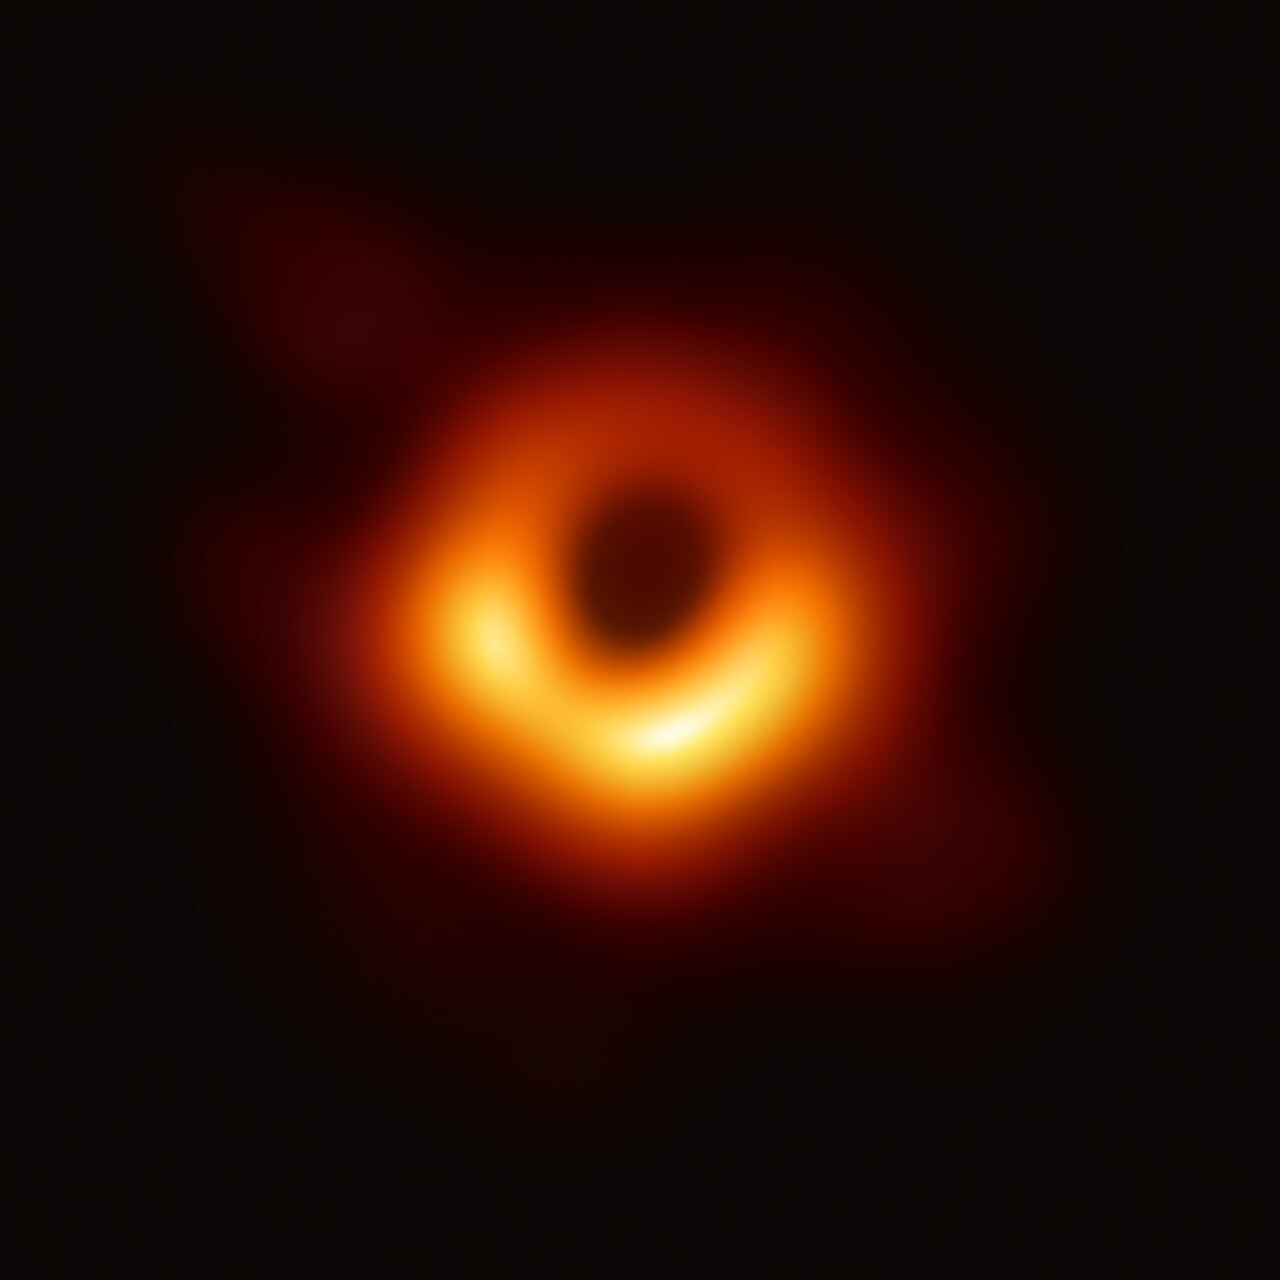
\includegraphics[height=\paperheight]{eht-photo.jpg}};
\fill[night,path fading=east] ([xshift=-\paperheight]current page.north east) rectangle ([xshift=-.6\paperheight]current page.south east);
\node[anchor=south west,font=\scriptsize,text=white!70,align=left] at ([xshift=.75cm,yshift=.45cm]current page.south west)
  {AI agents course (M.~Zaldarriaga \& N.~Mirón Granese)\\[1pt]
   {\tiny\color{white!50}FCEN--UBA \ \textperiodcentered{} \ 2 October 2026 \ \textperiodcentered{} \ \texttt{github.com/ddblanco/BHs}}};
\node[anchor=south east,font=\tiny,text=white!55] at ([xshift=-6pt,yshift=4pt]current page.south east) {M87*, Event Horizon Telescope (2019)};
\end{tikzpicture}%
\vspace*{.2cm}
\begin{minipage}{.62\textwidth}
{\scriptsize\bfseries\color{gold}\MakeUppercase{Gravitational Waves and AI-Assisted Research}\par}
\vspace{.35cm}
{\fontsize{26}{29}\selectfont\bfseries How hard can a\\black hole \textcolor{glow}{spin}?\par}
\vspace{.35cm}
{\small\color{white!80}Extremality shift of rotating black holes\\at finite Gauss--Bonnet coupling\par}
\vspace{.5cm}
{\footnotesize C.~Bejarano \ D.~Blanco \ A.~Goya \ G.~Pérez Nadal\par}
\vspace{.12cm}
{\scriptsize\color{white!65}with \textbf{\color{white}Claude Code} and \textbf{\color{white}Codex}\par}
\end{minipage}
\end{frame}

% ---------------------------------------------------------------- 2  problem
\begin{frame}[plain]\relax
\begin{columns}[c,onlytextwidth]
\column{.58\textwidth}
{\scriptsize\bfseries\color{gold}THE QUESTION\par}\vspace{6pt}
{\LARGE\bfseries There is a speed limit.\par}
\vspace{8pt}
{\small\color{white!80}Kerr (4D, GR): \ {\color{white}$M^2\ge|J|$}\par}\vspace{4pt}
{\small\color{white!80}Myers--Perry (5D, GR): \ {\color{white}$M\ge\tfrac32\,\pi^{1/3}J^{2/3}$}\par}
\vspace{4pt}
{\small\color{white}$\mathcal{L}=R+2\Lambda+\alpha\,(R^2-4R_{ab}^2+R_{abcd}^2)$\par}
\vspace{10pt}
{\small\color{white!80}Add Gauss--Bonnet, coupling $\alpha$: it moves.\\
Known only for tiny $\alpha$: \ slope $=\pi$.\par}
\vspace{14pt}
{\Large\bfseries And at \textcolor{glow}{finite} $\alpha$?\par}
\vspace{4pt}
{\small\color{white!80}Does the entropy of nearby black holes predict it?\par}
\column{.40\textwidth}\centering
\card{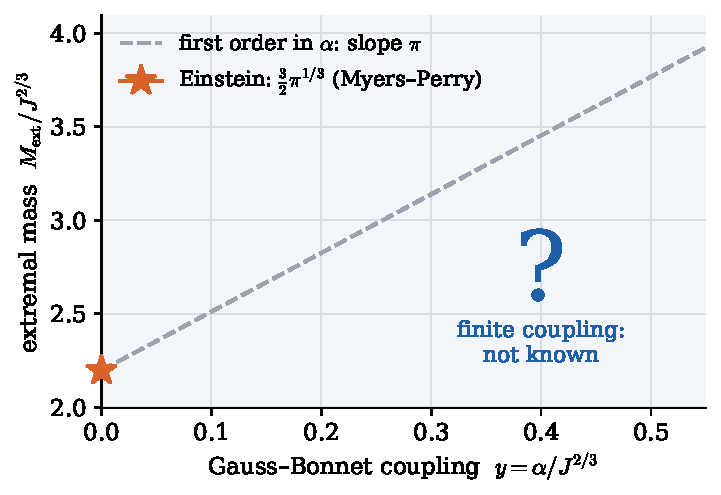
\includegraphics[width=\dimexpr\linewidth-10pt\relax]{fig-question.pdf}}
\end{columns}
\end{frame}

% ---------------------------------------------------------------- 3  result
\begin{frame}[plain]\relax
{\scriptsize\bfseries\color{gold}THE RESULT\par}\vspace{4pt}
{\LARGE\bfseries The limit gets \textcolor{glow}{tighter}.\par}
{\large\color{white!75}But not the way first order said.\par}
\vspace{8pt}
\begin{columns}[c,onlytextwidth]
\column{.58\textwidth}\centering
% Fixed-height right column (overlayarea) and equal card heights, so title and text do not move between overlays.
\only<1>{\card{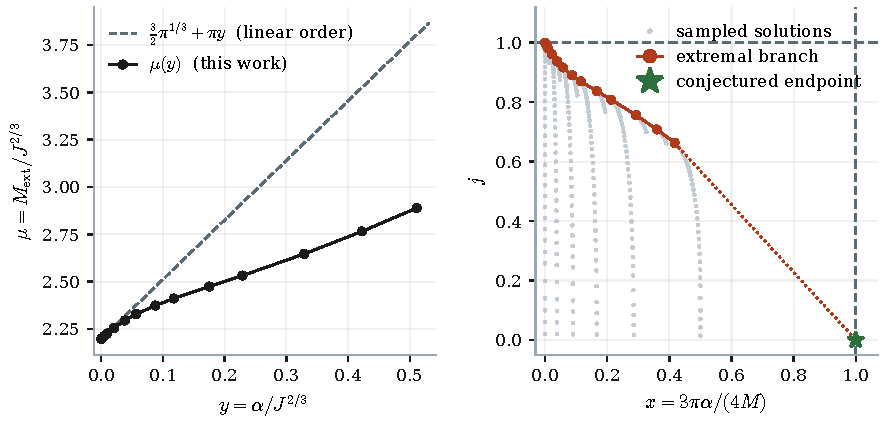
\includegraphics[height=4.7cm,trim=0 0 208.1bp 0,clip]{fig-massext.pdf}}}%
\only<2>{\card{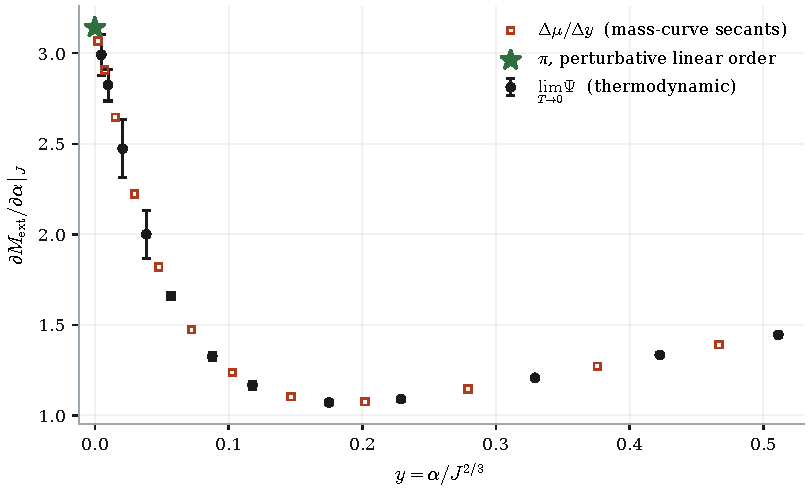
\includegraphics[height=4.7cm]{fig-shift.pdf}}}
\column{.40\textwidth}\centering
\begin{overlayarea}{\linewidth}{5.2cm}\centering
\only<1>{%
{\scriptsize\color{white!65}mass read at infinity, then $T\to0$ at fixed $J$\par}\vspace{2pt}
{\small$b\simeq1+U/r^2,\quad M=-\tfrac{3\pi}{8}\,U$\par}
\vspace{14pt}
{\fontsize{22}{26}\selectfont\bfseries\color{glow}$+31\%$\par}
{\scriptsize\color{white!65}growth of the extremal mass $M_\ext$\par}
\vspace{8pt}
{\fontsize{22}{26}\selectfont\bfseries $2.3\times$\par}
{\scriptsize\color{white!65}first order overshoots the real shift\par}}%
\only<2>{%
{\scriptsize\color{white!65}extended first law\par}\vspace{2pt}
{\small$dM=T\,dS+2\,\Omega_H\,dJ+\tikz[baseline=(x.base)]\node[draw=glow,rounded corners=2pt,inner sep=2pt,text=glow](x){$\Psi\,d\alpha$};$\par}
\vspace{4pt}
{\scriptsize\color{white!65}at $T=0$, fixed $J$: the entropy predicts the slope\par}\vspace{2pt}
{\small$\Psi_\ext=\left.\dfrac{\partial M_\ext}{\partial\alpha}\right|_J$\par}
\vspace{8pt}
{\fontsize{22}{26}\selectfont\bfseries\color{glow}$\pi\to1.07\to1.44$\par}
{\scriptsize\color{white!65}slope: falls, then rises\par}
\vspace{4pt}
{\scriptsize\color{white!65}$\Psi$ (dots) and mass at infinity (squares) agree: worst interval $0.2\%$\par}}
\end{overlayarea}
\end{columns}
\end{frame}

% ---------------------------------------------------------------- 4  validation
\begin{frame}[plain]\relax
\begin{columns}[c,onlytextwidth]
\column{.42\textwidth}
{\scriptsize\bfseries\color{gold}WHY BELIEVE IT\par}\vspace{6pt}
{\fontsize{54}{56}\selectfont\bfseries\color{glow}10\par}
{\Large\bfseries independent checks.\par}
\vspace{6pt}
{\large All below $10^{-4}$.\par}
\vspace{14pt}
{\small\color{white!75}\alert<2>{Known solutions first:} arXiv:1010.0860 to $2\times10^{-4}$.\\[3pt]
$\Psi$ three ways (first law, Smarr relation, Gauss--Bonnet action)
agrees to $\sim10^{-6}$: a test of our entropy and charges.\par}
\vspace{8pt}
{\scriptsize\color{white!55}Largest uncertainty: the $T\to0$ extrapolation.\par}
\column{.55\textwidth}\centering
\only<1,3>{\card{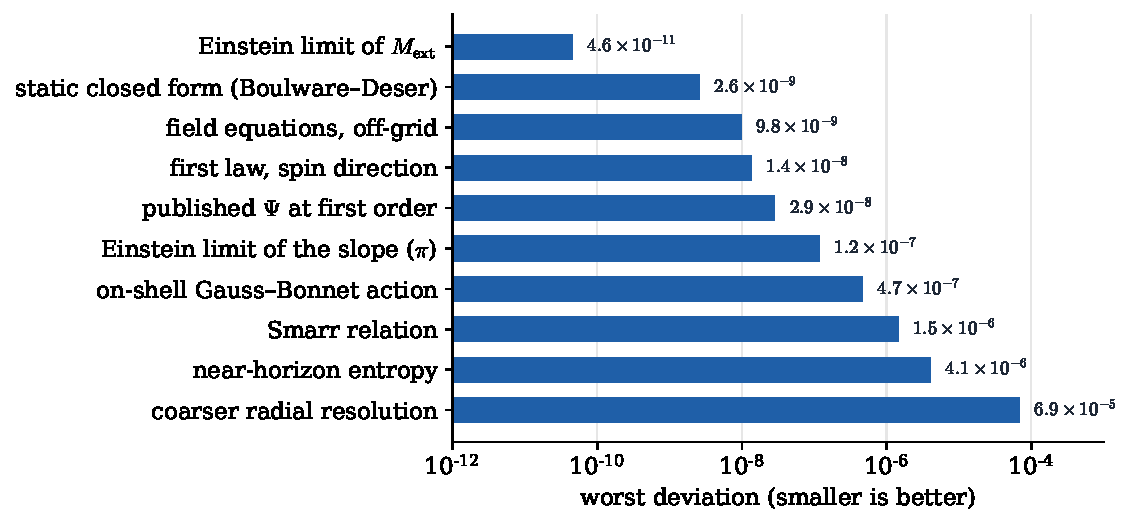
\includegraphics[width=\dimexpr\linewidth-10pt\relax]{fig-checks.pdf}}}%
\only<2>{\card{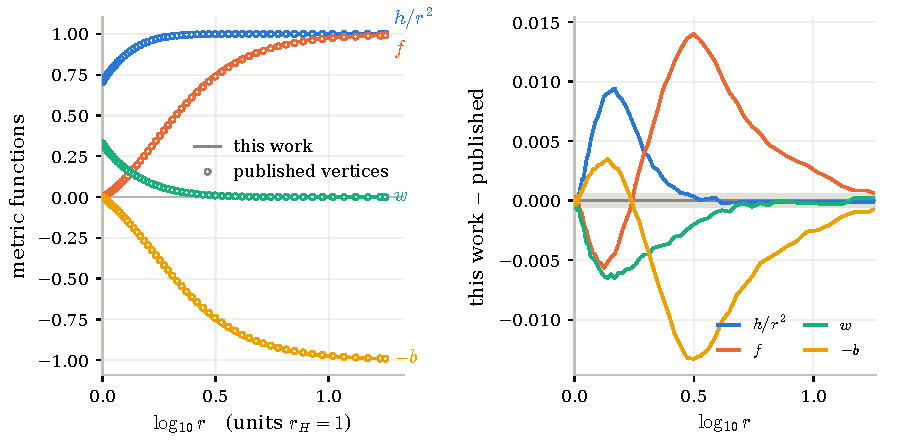
\includegraphics[height=4.9cm,trim=0 0 217bp 0,clip]{fig-paper-comparison.pdf}}\par\vspace{3pt}
{\scriptsize\color{white!65}lines: our solver \quad circles: arXiv:1010.0860, fig.~1\par}}
\end{columns}
\end{frame}

% ---------------------------------------------------------------- 5  experience
\begin{frame}[plain]\relax
\centering
{\scriptsize\bfseries\color{gold}HOW IT WAS MADE \& WHAT WE LEARNED\par}\vspace{6pt}
{\LARGE\bfseries Two AI agents. One of them the \textcolor{glow}{referee}.\par}
\vspace{18pt}
\begin{columns}[T,onlytextwidth]
\column{.33\textwidth}\centering{\fontsize{30}{34}\selectfont\bfseries 36.8\,h\par}{\scriptsize\color{white!65}agent time, 13 days\par}
\column{.34\textwidth}\centering{\fontsize{30}{34}\selectfont\bfseries 1.42\,B\par}{\scriptsize\color{white!65}tokens processed\par}
\column{.33\textwidth}\centering{\fontsize{30}{34}\selectfont\bfseries 79\par}{\scriptsize\color{white!65}human prompts\par}
\end{columns}
\vspace{18pt}
{\scriptsize\color{white!55}(4.4\,h reproducing, 11.2\,h new solver, 8.7\,h $\Psi_{T\to0}$)\par}
\vspace{8pt}
{\large Writing the code was cheap.\par}
{\Large\bfseries\color{glow}Verifying it was the work.\par}
\end{frame}

% ================================================================ after the talk
% \appendix here so that the frame total counts only slides 1-5.
\appendix

% ---------------------------------------------------------------- 6  thanks
\begin{frame}[plain]\relax
\begin{tikzpicture}[remember picture,overlay]
\node[inner sep=0] at (current page.center) {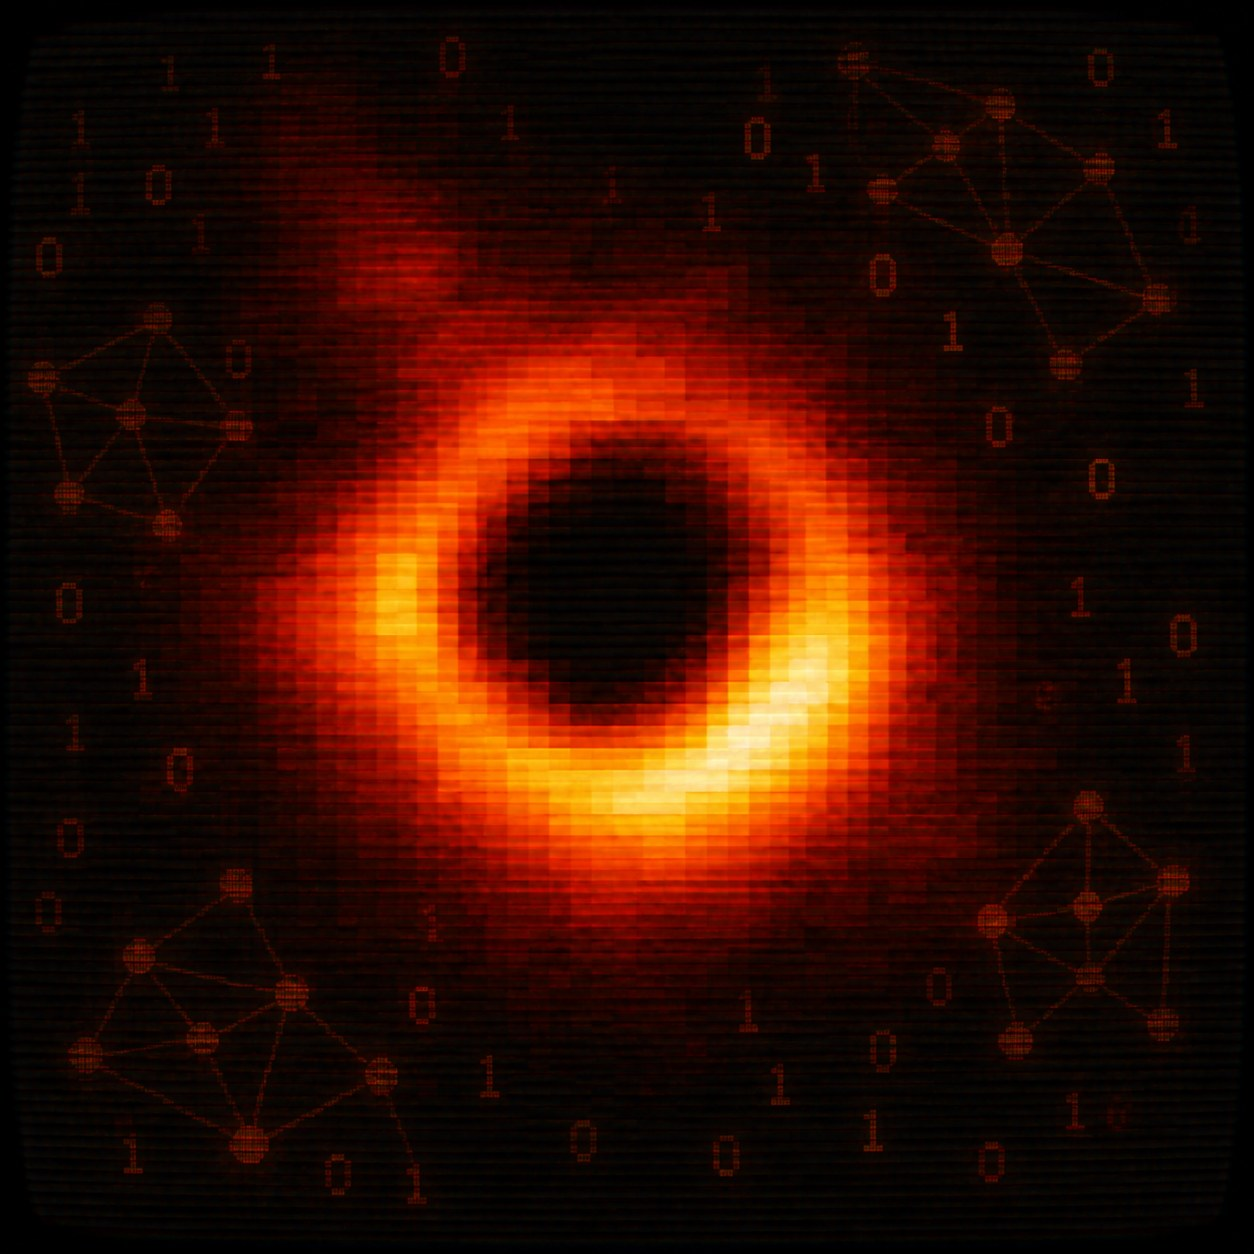
\includegraphics[height=\paperheight]{retro-crt.jpg}};
\fill[night,opacity=.45] (current page.south west) rectangle (current page.north east);
% Fade the square image's left and right edges into the night background of the other slides.
\fill[night,path fading=east] ([xshift=-.5\paperheight]current page.north) rectangle ([xshift=-.25\paperheight]current page.south);
\fill[night,path fading=west] ([xshift=.25\paperheight]current page.north) rectangle ([xshift=.5\paperheight]current page.south);
\end{tikzpicture}%
Thank you for your attention\\[14pt]
{\normalsize\mdseries Matías and Nahuel, thanks for the AI course}
\end{frame}

% ================================================================ backup

% ---------------------------------------------------------------- A1
\begin{frame}{A1 \textperiodcentered{} Numerical method: solving the field equations}
\vspace{-6pt}
\begin{columns}[T,onlytextwidth]
\column{.53\textwidth}\scriptsize
\setlength{\abovedisplayskip}{1pt}\setlength{\belowdisplayskip}{1pt}
{\bfseries\color{accent}Equal-spin ansatz} $\Rightarrow$ ODEs in $r$ for $b,f,h,w$:
\[\begin{aligned}ds^2={}&-b\,dt^2+\frac{dr^2}{f}+r^2\bigl[d\theta^2+\sin^2\!\theta\cos^2\!\theta\,(d\varphi_1-d\varphi_2)^2\bigr]\\
&+h\,\bigl[\sin^2\!\theta\,d\varphi_1+\cos^2\!\theta\,d\varphi_2-w\,dt\bigr]^2\end{aligned}\]
horizon: $b=f=0$, $w=\Omega_H$;\ \ infinity: $b,f,h/r^2\to1$, $w\to0$\par
\column{.45\textwidth}\scriptsize
{\bfseries\color{accent}Discretise:} $\chi=1-r_H/r$, Chebyshev--Lobatto, $N=64$:
$R_N(u;\alpha,r_H,\Omega_H)=0$ \ ($4N$ eqs.)\\[2pt]
{\bfseries\color{accent}Solve:} damped Newton; continuation from Myers--Perry\\[2pt]
{\bfseries\color{accent}Accept:} $G_{\mu\nu}+\alpha H_{\mu\nu}<10^{-8}$ at 51 off-grid points\\[2pt]
{\bfseries\color{accent}Read off:} $b\simeq1+U/r^2$, $w\simeq W/r^4$ $\Rightarrow$ $M=-\tfrac{3\pi}8U$, $J=\tfrac\pi4W$
\end{columns}
\vspace{4pt}
\begin{columns}[T,onlytextwidth]
\column{.43\textwidth}\centering
\card{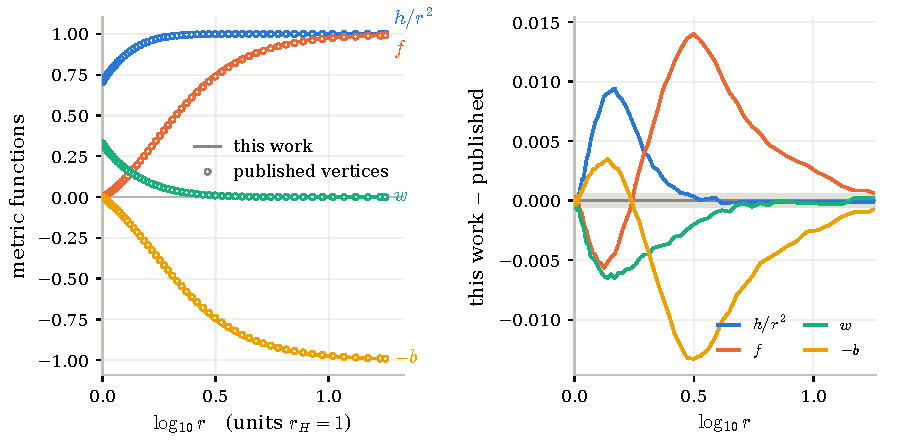
\includegraphics[height=3.6cm,trim=0 0 217bp 0,clip]{fig-paper-comparison.pdf}}
\column{.55\textwidth}\centering
\card{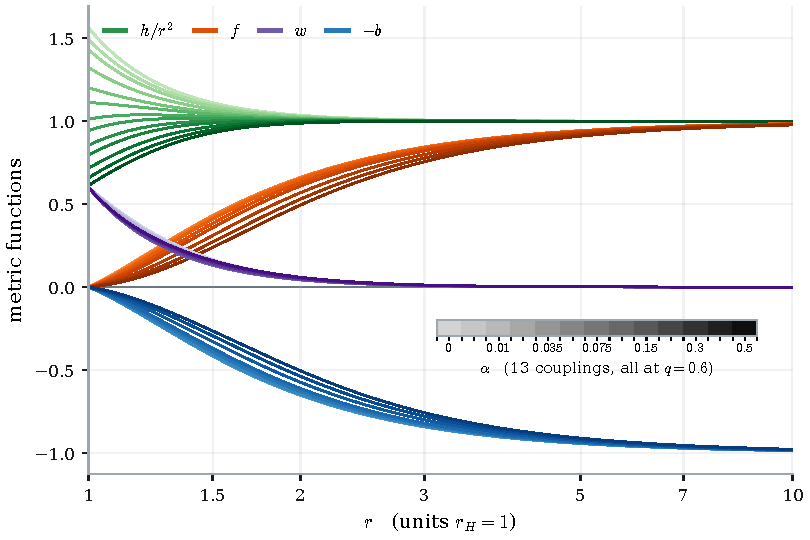
\includegraphics[height=3.6cm]{fig-profiles.pdf}}
\end{columns}
\end{frame}

% ---------------------------------------------------------------- A2
\begin{frame}{A2 \textperiodcentered{} Numerical method: measuring $\Psi$ and reaching $T=0$}
\begin{columns}[T,onlytextwidth]
\column{.47\textwidth}\small
\hd{$\Psi$ from derivatives at fixed $(r_H,\Omega_H)$}
\[\Psi=\left.\frac{\partial M}{\partial\alpha}\right|_{S,J}=M_\alpha-T\,S_\alpha-2\Omega_H\,J_\alpha\]

\hd{Derivatives without finite differences}
\[\underbrace{\frac{\partial R_N}{\partial u}}_{\mathclap{\text{Newton Jacobian}}}\frac{du}{d\alpha}=-\frac{\partial R_N}{\partial\alpha}\]
\scriptsize one linear solve, no step size (implicit function theorem)

\medskip\small
\hd{Get cold, then extrapolate}\\
cubic fit through the 6 coldest states;\\
coldest $TJ^{1/3}\approx3\times10^{-6}$

\smallskip\scriptsize\color{muted}$M_\ext$ is read at infinity; $\Psi_{T\to0}$ is the slope the entropy predicts.
\column{.51\textwidth}\centering
\card{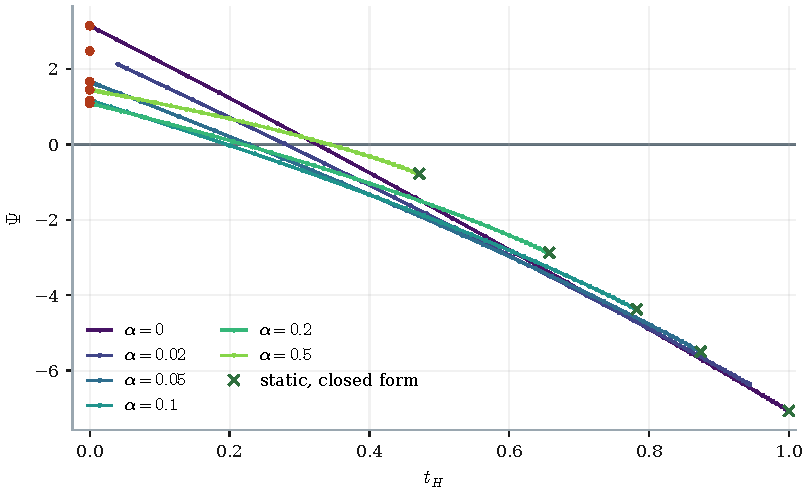
\includegraphics[width=\dimexpr\linewidth-10pt\relax]{fig-potential.pdf}}\\
\scriptsize $\Psi$ against temperature; red dots: the $T=0$ values (the slope)
\end{columns}
\end{frame}

% ---------------------------------------------------------------- A2b
% manuscript/main.tex, paragraphs "The potential from the Smarr relation" and
% "The potential as an on-shell action"; numbers from manuscript/numbers.tex.
\begin{frame}{A2b \textperiodcentered{} Two other routes to $\Psi$}
\begin{columns}[T,onlytextwidth]
\column{.48\textwidth}\small
\setlength{\abovedisplayskip}{3pt}\setlength{\belowdisplayskip}{3pt}
\hd{1. Smarr relation} \src{(scaling)}\\
weights: $M,\alpha\to2$, \ $S,J\to3$; Euler's theorem:
\[2M=3TS+6\Omega_HJ+2\alpha\Psi\]
\[\Rightarrow\quad\Psi=\frac{2M-3TS-6\Omega_HJ}{2\alpha}\]
\scriptsize charges of \alert{one} solution: no Jacobian, no derivative\\[2pt]
agrees to $1.45\times10^{-6}$ (313 states);\ useless as $\alpha\to0$
\column{.48\textwidth}\small
\setlength{\abovedisplayskip}{3pt}\setlength{\belowdisplayskip}{3pt}
\hd{2. On-shell Gauss--Bonnet action}\\
Gibbs potential = on-shell action per unit time; at fixed $(T,\Omega_H)$, $\alpha$ enters explicitly only through $\mathcal L_\GB$ (field equations remove the rest):
\[\Psi=-\frac1{16\pi}\int_\Sigma\!\sqrt{-g}\,\mathcal L_\GB\]
\scriptsize curvature of the solution only: no charge extraction either\\[2pt]
agrees to $4.67\times10^{-7}$ (43 states, away from extremality)
\end{columns}
\vfill
\centering\src{Smarr is the first law plus scaling: the same law along another path.
Both use the same numerical solutions; neither uses the linear solve of A2.}
\end{frame}

% ---------------------------------------------------------------- A3
\begin{frame}{A3 \textperiodcentered{} Physical meaning of the result}
\centering
\card{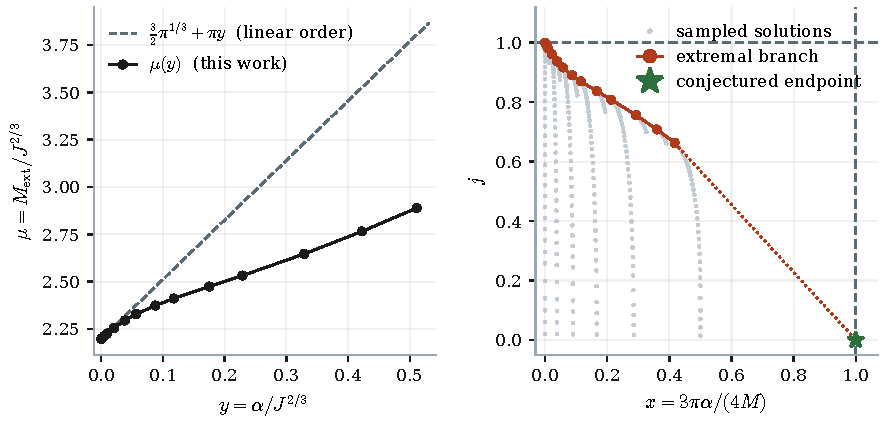
\includegraphics[width=.62\textwidth]{fig-massext.pdf}}

\vspace{2pt}
\begin{columns}[T,onlytextwidth]
\column{.34\textwidth}\centering\small
\hd{Spin bound}\\
$\Psi_\ext>0\ \Leftrightarrow\ j_\ext$ falls:\\
less spin per unit mass
\column{.32\textwidth}\centering\small
\hd{Slope minimum}\\
$3\omega=\mu-y\,\mu'$\\
= fastest extremal horizon,\\ $\omega=\Omega_HJ^{1/3}$
\column{.34\textwidth}\centering\small
\hd{Why it rises again}\\
$M>\tfrac{3\pi}4\alpha$ \ forces\\
$\mu'\to\tfrac{3\pi}{4}\approx2.36$
\end{columns}
\end{frame}

% ---------------------------------------------------------------- A4
\begin{frame}[t]{A4 \textperiodcentered{} How it started: the first prompts}
\vspace{-4pt}
\begin{beamercolorbox}[wd=\linewidth,sep=4pt,leftskip=4pt]{block body}
\scriptsize\itshape ``El proyecto consiste en utilizar agentes de IA para implementar códigos
numéricos que permitan obtener soluciones de agujeros negros rotantes en
dimensión D>4 [\ldots] reproducir soluciones numéricas ya encontradas en la
literatura. [\ldots] el paso siguiente sería emprender la búsqueda de nuevas
soluciones.''\par\smallskip\upshape\tiny\color{muted}Prompt 1 --- 4 Sept, 19:16, to Codex
\quad\textperiodcentered{}\quad then ``Fijate que el proyecto realmente siga las indicaciones propuestas por el
docente del curso'' (3), ``ejecutar con subagentes'' (5), ``continuemos con el hito 3'', ``dale, avanzá''
\quad\textperiodcentered{}\quad \textbf{79} human prompts, 4--28 Sept \quad\textperiodcentered{}\quad Claude Code builds $\leftrightarrow$ Codex referees
\end{beamercolorbox}
\par\vspace{-16pt}\noindent
\begin{minipage}[t]{.44\textwidth}\vspace{0pt}\centering
\card{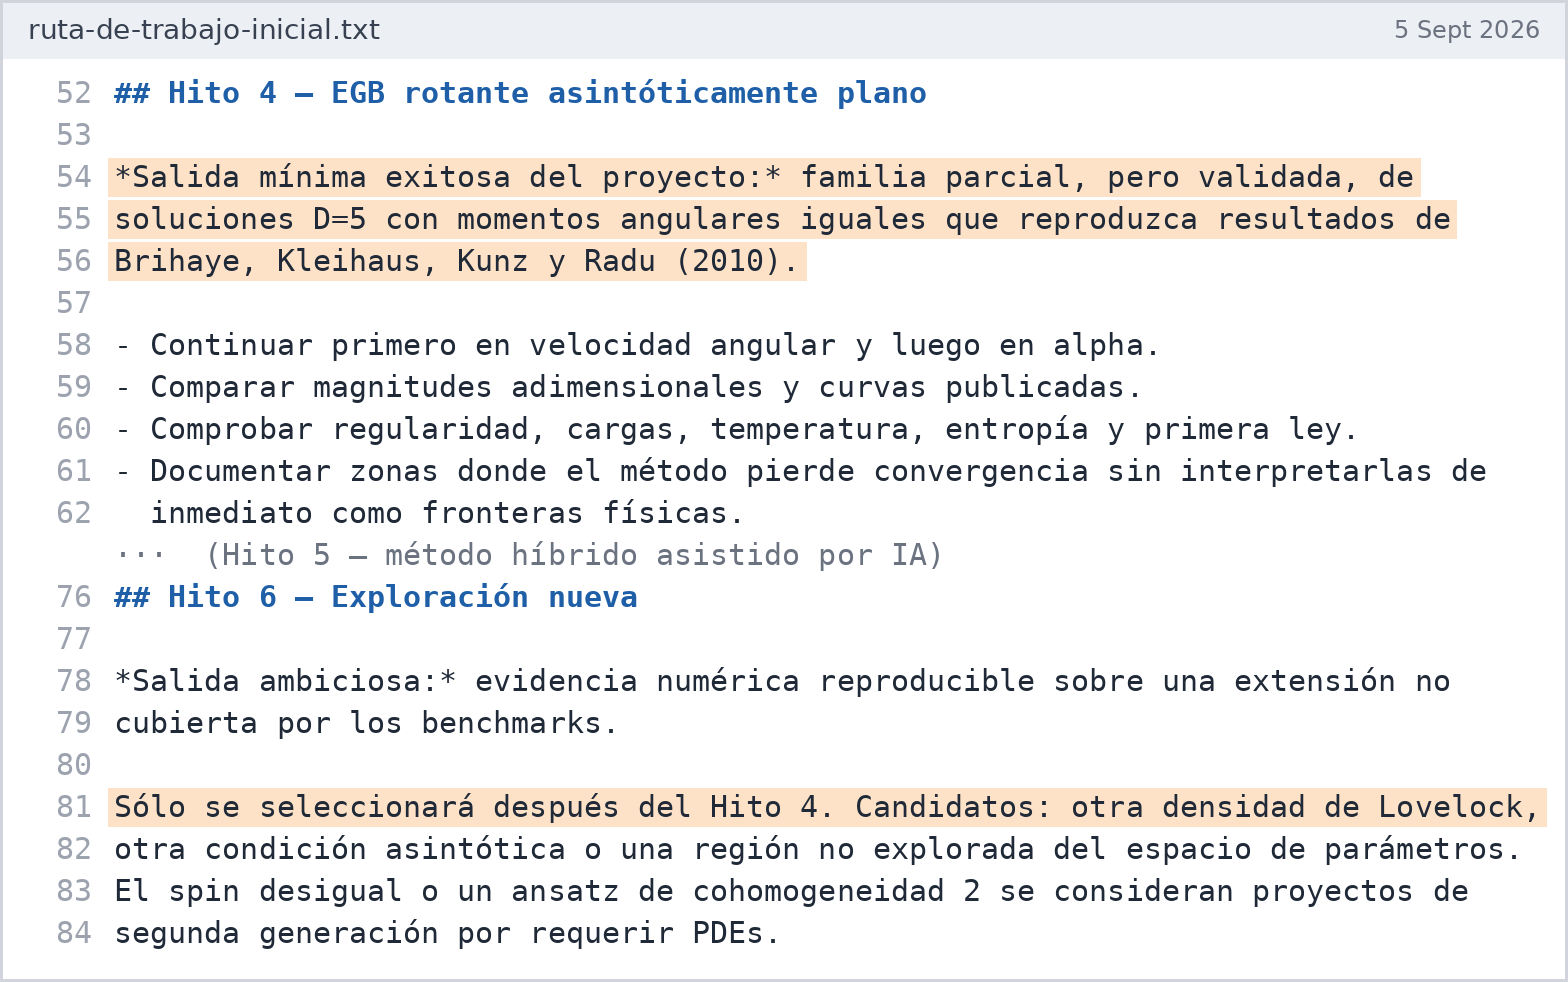
\includegraphics[width=.84\linewidth]{fig-roadmap.png}}\par\vspace{2pt}
{\tiny\color{muted}first roadmap, 5 Sept. \textcolor{glow}{Hito 6} became $\Psi$;
Hito 8 ($T\to0$, paper, referees) was not in the plan.\par}
\end{minipage}\hfill
\begin{minipage}[t]{.52\textwidth}\vspace{0pt}\centering
\card{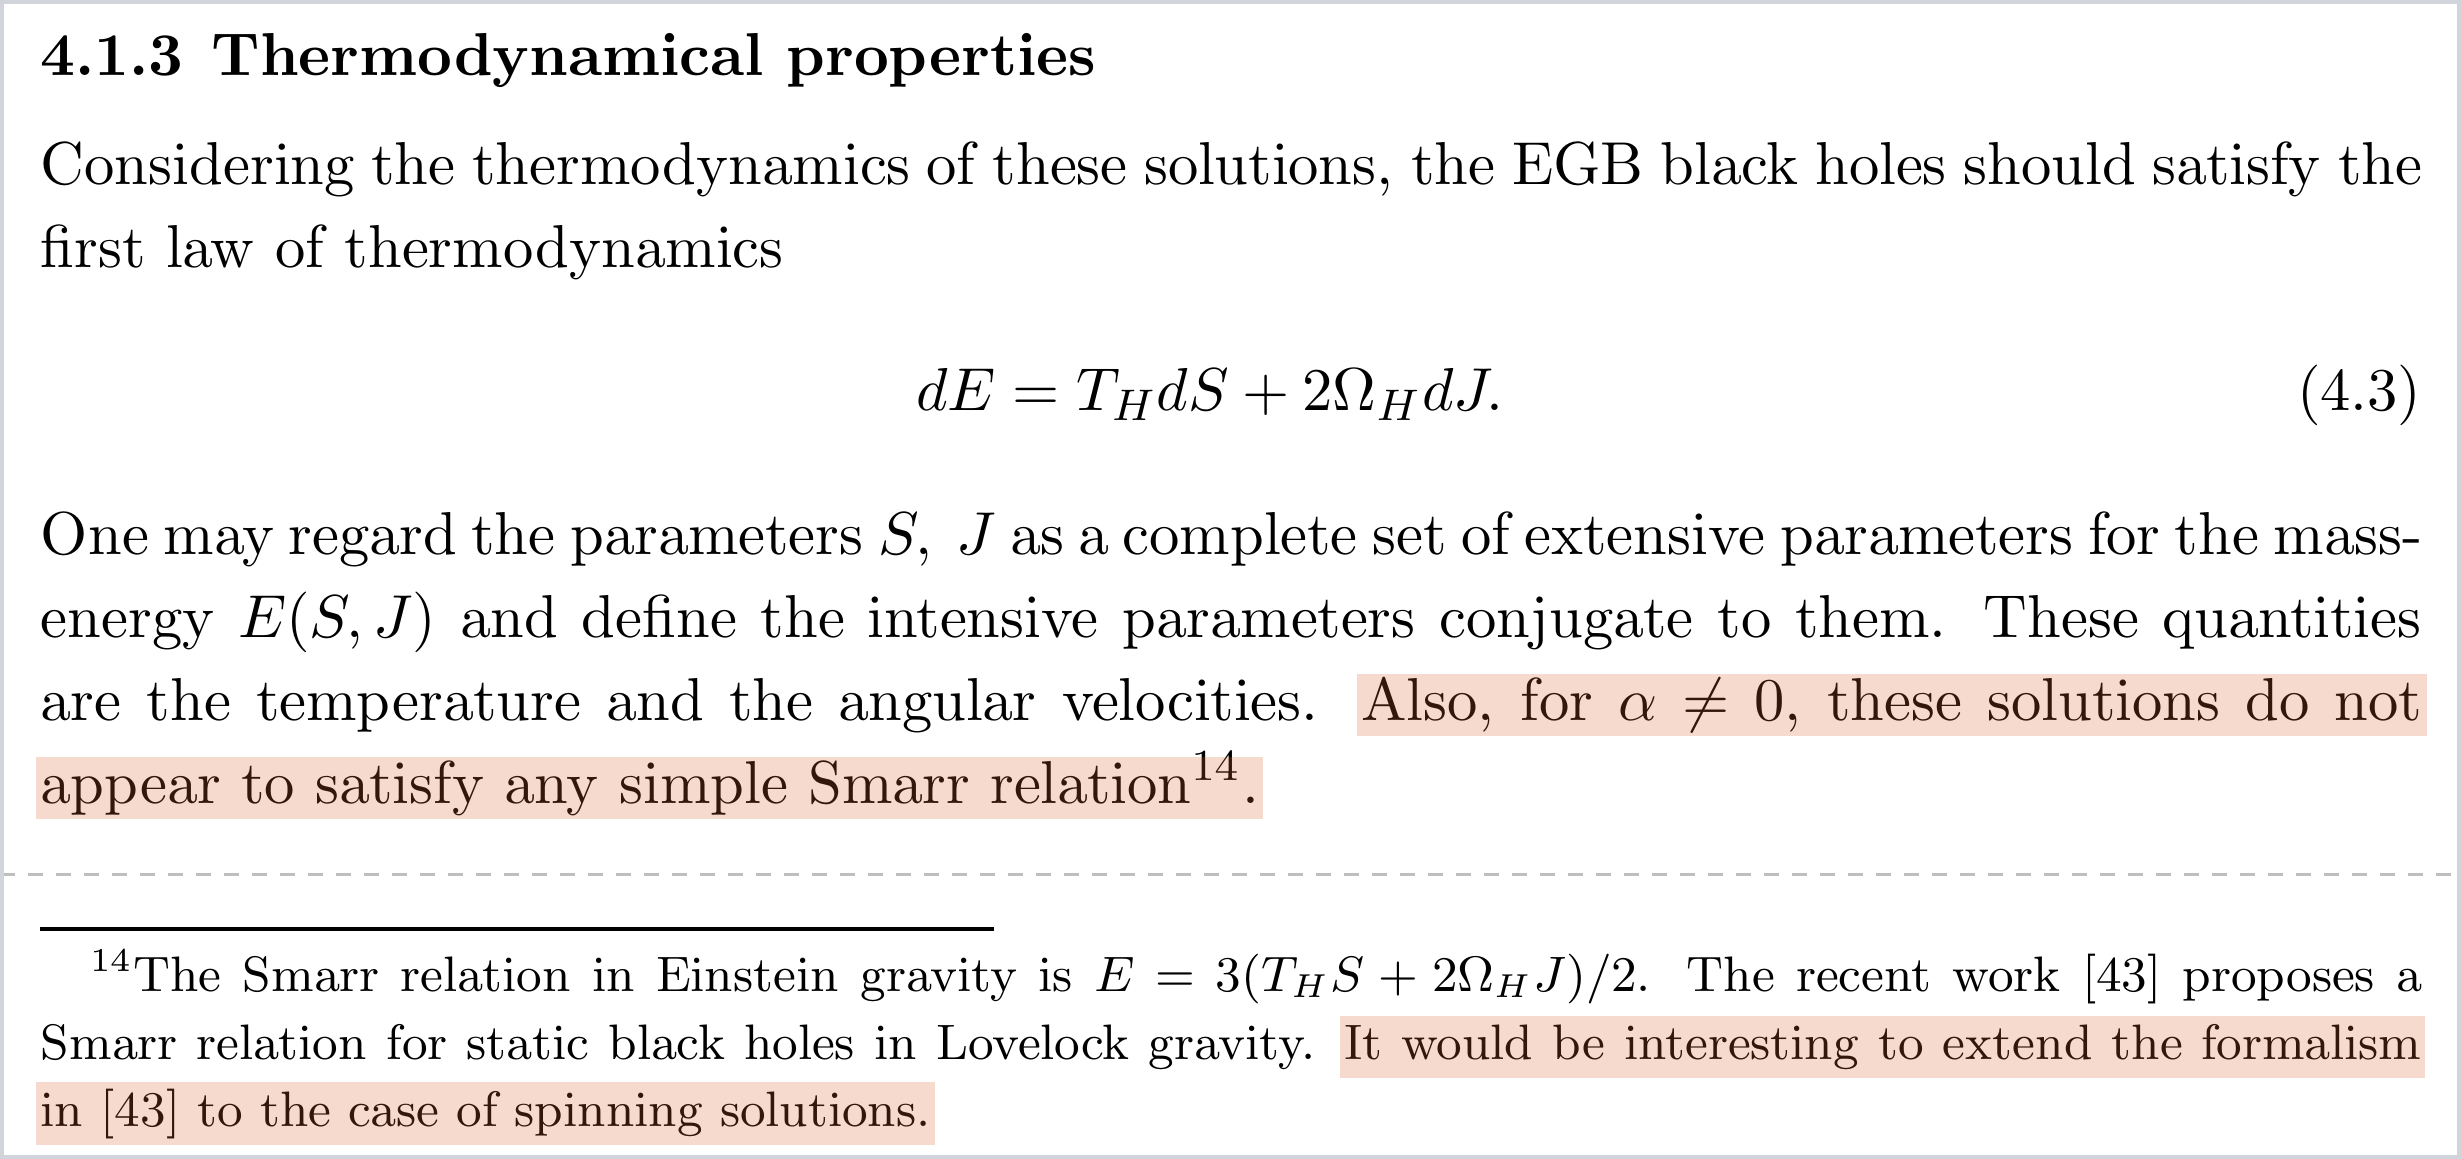
\includegraphics[width=.9\linewidth]{fig-smarr.png}}\par\vspace{2pt}
{\tiny\color{muted}arXiv:1010.0860, \S4.1.3 and footnote 14.\par}
\vspace{4pt}
{\scriptsize Hito 6, $\alpha$ as a thermodynamic variable:\
$2M=3TS+6\Omega_HJ+2\alpha\Psi$\par}
\end{minipage}
\end{frame}

% ---------------------------------------------------------------- A5
\begin{frame}{A5 \textperiodcentered{} What it cost}
\centering
\begin{columns}[T,onlytextwidth]
\column{.25\textwidth}\centering\stat{36.8 h}{active agent time, 13 days}
\column{.25\textwidth}\centering\stat{1.42 billion}{tokens processed\\(99\% re-read context)}
\column{.25\textwidth}\centering\stat{5.9 million}{tokens written ($\approx$24 MB)}
\column{.25\textwidth}\centering\stat{79}{human prompts}
\end{columns}
\vspace{4pt}
\card{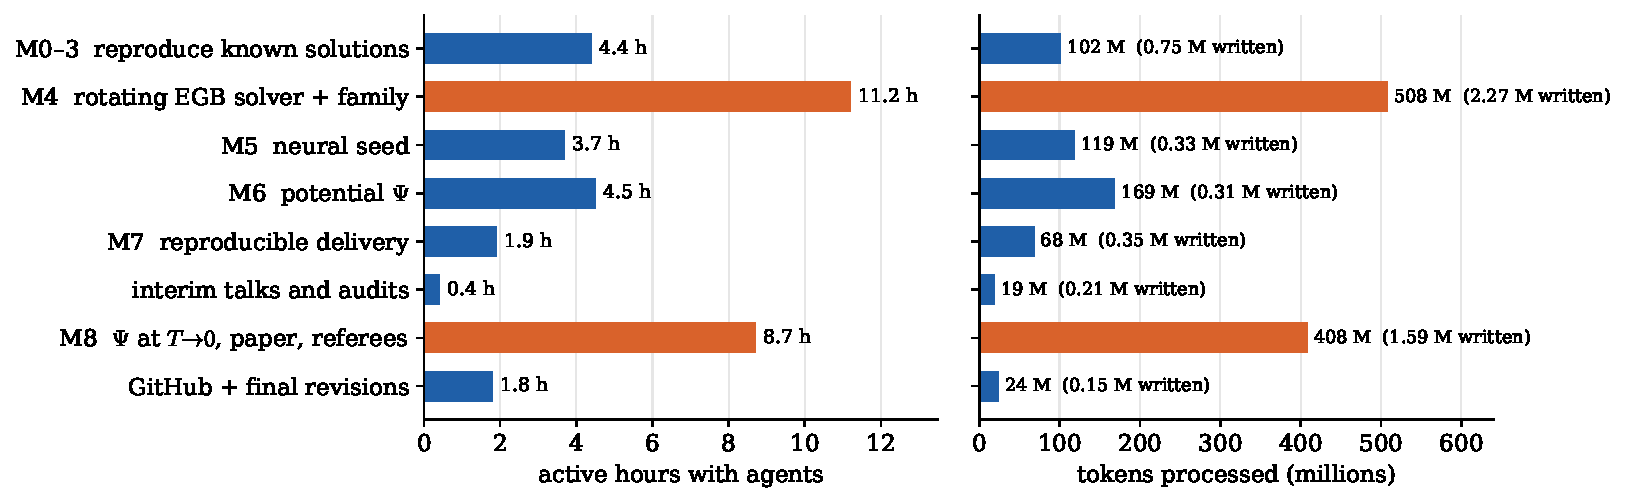
\includegraphics[width=.8\textwidth]{fig-cost.pdf}}\\
\small The first \alert{new} object cost $5\times$ the tokens of reproducing everything known.\\[2pt]
\src{Not counted: human time, background numerical runs.}
\end{frame}

\end{document}
